\documentclass{beamer}

% biber

\usepackage[brazilian]{babel}
\usepackage[utf8]{inputenc}
\usepackage{graphicx}
\usepackage{mathtools}
\usepackage{amsthm}
\usepackage{thmtools,thm-restate}
\usepackage{amsfonts}
\usepackage{amssymb}
\usepackage{hyperref}
\usepackage[backend=biber,url=true,doi=true,eprint=false,style=alphabetic]{biblatex}
\usepackage{enumitem}
\usepackage[justification=centering,singlelinecheck=false]{caption}
\usepackage{indentfirst}
\usepackage{tikz}
\usepackage{hyperref}
\usepackage{subcaption}
\usepackage{booktabs}
\usepackage{linegoal}
\usepackage{csquotes}
\usetikzlibrary{snakes,arrows,shapes}

\addbibresource{references.bib}

\setitemize{label=\usebeamerfont*{itemize item}%
  \usebeamercolor[fg]{itemize item}
\usebeamertemplate{itemize item}}

\setenumerate[1]{%
  label=\protect\usebeamerfont{enumerate item}%
        \protect\usebeamercolor[fg]{enumerate item}%
        \insertenumlabel.}

\uselanguage{brazilian}
\languagepath{brazilian}
\deftranslation[to=brazilian]{theorem}{teorema}
\deftranslation[to=brazilian]{Theorem}{Teorema}
\deftranslation[to=brazilian]{Definition}{Definição}
\deftranslation[to=brazilian]{definition}{definição}
\deftranslation[to=brazilian]{Lemma}{Lema}
\deftranslation[to=brazilian]{lemma}{lema}
\deftranslation[to=brazilian]{Example}{Exemplo}
\deftranslation[to=brazilian]{example}{exemplo}
\usetheme{boxes}

\setbeamertemplate{bibliography entry title}{}
\setbeamertemplate{bibliography entry location}{}
\setbeamertemplate{bibliography entry note}{}

\setbeamertemplate{theorems}[ams style]
\setbeamertemplate{caption}[numbered]{}

\DeclareMathOperator*{\argmin}{arg\,min}
\DeclareMathOperator*{\argmax}{arg\,max}
\DeclareMathOperator*{\Val}{\text{Val}}
\DeclareMathOperator*{\Ch}{\text{Ch}}
\DeclareMathOperator*{\Pa}{\text{Pa}}
\DeclareMathOperator*{\Sc}{\text{Sc}}
\DeclareMathOperator*{\PoA}{\text{PoA}}
\newcommand{\cls}{\hat{C}}
\newcommand{\ov}{\overline}
\newcommand{\region}{\mathcal}

\captionsetup[table]{labelsep=space}

\theoremstyle{plain}

\newtheorem{lemma-cnt}{Lema}
\newtheorem{proposition}{Proposição}
\newtheorem{exercise}{Exercício}

\newcommand{\set}[1]{\mathbf{#1}}
\newcommand{\pr}{\mathbb{P}}
\newcommand{\eps}{\varepsilon}
\renewcommand{\implies}{\Rightarrow}
\newcommand{\gadget}{\textit{gadget}}
\newcommand{\bcolor}[1]{{\color{blue} #1}}

\setlength{\parskip}{1em}

\newcommand{\code}[1]{\lstinline[mathescape=true]{#1}}
\newcommand{\mcode}[1]{\lstinline[mathescape]!#1!}

\newcommand{\p}{\pause}

\title{Jogos de Anti-Coordenação e Colorações Estáveis em Grafos}
\author{Renato Lui Geh\\NUSP:8536030}
\date{}

\begin{document}

\frame{\titlepage}

\section{Introdução}
\begin{frame}
  \frametitle{Introdução}

  \begin{block}{Jogos de coordenação:}
    Classe de jogos em que jogadores jogam cooperativamente. Jogador $i$ fazer a mesma ação que
    jogador $j$ gera um benefício para ambos jogadores.
  \end{block}

  \begin{block}{Exemplos:}
    \begin{itemize}
      \item Batalha dos sexos (visto em aula)
      \item Caça ao cervo
    \end{itemize}
  \end{block}
\end{frame}

\begin{frame}
  \begin{block}{Jogos de anti-coordenação:}
    Variante do jogo de coordenação em que jogador $i$ escolher mesma ação que jogador $j$ gera
    custo.
  \end{block}

  \begin{block}{Exemplos:}
    \begin{itemize}
      \item Mineração
      \item Habilidades de empregados
      \item Rotas de avião
    \end{itemize}
  \end{block}
\end{frame}

\begin{frame}
  \begin{block}{Dois jogadores:}
    \begin{itemize}
      \item Fácil
      \item Matriz de utilidade/custo
    \end{itemize}
  \end{block}

  \begin{block}{Mais de dois jogadores:}
    \begin{itemize}
      \item Difícil
      \item Grafos
    \end{itemize}
  \end{block}
\end{frame}

\begin{frame}
  \textbf{Jogo:} $G=(V,E)$\\
  \begin{align*}
    v\in V:\quad &\text{jogador}\\
    e\in E:\quad &\text{relação entre dois jogadores}\\
    \{1,\ldots,k\}:\quad &\text{ações}\\
  \end{align*}
  \textbf{Utilidade:} número de vizinhos que têm ações diferentes\\
  \textbf{Equilíbrio:} $v$ não tem incentivo para mudar ação dados vizinhos\\~\\

  Parece com algo?\p{} \textbf{Coloração}
\end{frame}

\begin{frame}
  \frametitle{Objetivos:}
  \begin{enumerate}
    \item Para $k\geq 2$, existe algoritmo polinomial para achar $k$-coloração estável num grafo
      não-direcionado.
    \item PoA para $k$-coloração em grafos não-direcionado é $\Theta\left(\frac{k}{k-1}\right)$.
    \item Para $k\geq 2$, descobrir se existe $k$-coloração estritamente estável num grafo
      não-direcionado é NP-difícil.
  \end{enumerate}

  Existe generalização do 3 para digrafos, mas vou mostrar apenas para grafos não-direcionados.
  Vejam~\cite{kun-et-al} se estiverem curiosos.
\end{frame}

\section{Definições}

\begin{frame}
  \frametitle{Definições}
  Seja $G=(V,E)$ grafo não-direcionado.\\
  Chamamos $c\in C=\{f|f:V\to\{1,\ldots,k\}\}$ de uma coloração.\\~\\

  Todos $v\in V$ escolhem cor simultaneamente. A utilidade de $v$ é:

  \begin{equation*}
    \mu_c(v) \coloneqq \sum_{\{u,v\}\in E} 1_{\{c(u)\neq c(v)\}}
  \end{equation*}

  O bem-estar social de $G$ dada uma coloração $c$ é:

  \begin{equation*}
    W(G,c)\coloneqq\sum_{v\in V}\mu_c(v)
  \end{equation*}
\end{frame}

\begin{frame}
  Uma coloração $c$ é \textbf{estável} se nenhum vértice $v$ pode aumentar $\mu_c(v)$ mudando
  $c(v)$.\\~\\

  Uma coloração $c$ é \textbf{estritamente estável} se para todo $v\in V$, toda $c'\in C$, $c'\neq
  c$ temos que $\mu_c(v)>\mu_{c'}(v)$. Senão, $c$ é \textbf{não-estrita}.\\~\\

  O PoA de $G$ é:

  \begin{equation*}
    \PoA(G)\coloneqq\frac{\max_{c'\in C} W(G,c')}{\min_{c\in Q} W(G,c)}
  \end{equation*}

  onde $Q$ é o conjunto de colorações estáveis.
\end{frame}

\begin{frame}
  \begin{figure}[h]
    \centering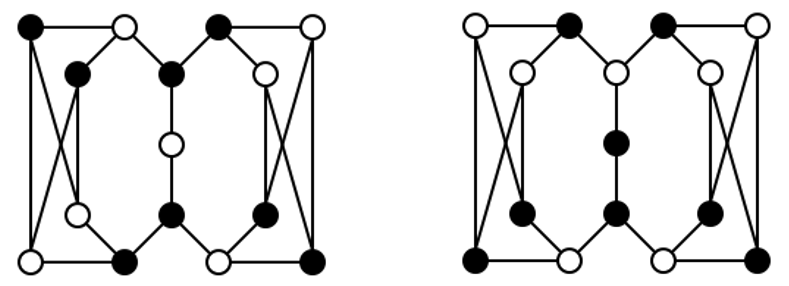
\includegraphics[scale=0.3]{imgs/ex1.png}
    \captionsetup{justification=raggedright}
    \caption{O grafo da esquerda é estritamente estável e tem $W(G,c)=40$, enquanto que o da
    direita é não-estrito com $W(G,c')=42$. Fonte:~\cite{kun-et-al}}
  \end{figure}
\end{frame}

\begin{frame}
  \frametitle{Colorações estáveis}
  \begin{proposition}\label{prop-1} Para todo $k\geq 2$, todo grafo finito $G=(V,E)$ admite uma
    $k$-coloração estável. Tal $k$-coloração estável pode ser encontrada em tempo polinomial.
  \end{proposition}
\end{frame}

\begin{frame}
  \frametitle{Demonstração (Proposição 1)}
  Primeiro chamaremos:
  \begin{align*}
    c:\quad &\text{coloração}\\
    \phi(c):\quad &\text{número de arestas coloridas apropriadamente}
  \end{align*}
  Note que $0\leq \phi(c)\leq |E|$. Vamos primeiro mostrar que $W(G,c)=2\phi(c)$.\\~\\
  Fixa $v\in V$.
  \begin{align*}
    &n_v:\quad \text{número de cores diferentes em $v$}\\
    &\phi(c)=\sum_{e\in E}1_{\{e\text{ apropriado}\}}
  \end{align*}
  Se $e$ é apropriado ($c(u)\neq c(v)$), então contamos $e$ duas vezes: $(u,v)$ e $(v,u)$.
\end{frame}

\begin{frame}
  Somando todas as arestas apropriadas para todo $v$:
  \begin{equation*}
    \sum_{v\in V}\sum_{e=\{u,v\}\in E}1_{\{e\text{ apropriado}\}}=\sum_{v\in V}n_v=2\phi(c)
  \end{equation*}
  Mas $n_v$ é exatamente $\mu_c(v)$.
  \begin{equation*}
    \sum_{v\in V}n_v=2\phi(c)=\sum_{v\in V}\mu_c(v)=W(G,c)
  \end{equation*}
  Note que $\phi(c)$ é uma função potencial exata, então esse é um jogo de potencial.
\end{frame}

\begin{frame}
  Dada uma coloração $c$, um vértice $v$ está \textit{infeliz} se $v$ tem mais vizinhos com mesma
  cor que $v$ do que diferentes.

  Para acharmos uma $k$-coloração estável em $G$ fazemos:

  Enquanto existe algum vértice $v$ infeliz, mude $c(v)$ para algum $c'(v)$ tal que
  \begin{equation*}
    c'(v)=\argmin_{m\in\{1,\ldots,k\}}\sum_{u\in N(v)}1_{\{c(u)=m\}},
  \end{equation*}
  onde $N(v)$ são os vizinhos de $v$.
\end{frame}

\begin{frame}
  Se $v$ é vértice infeliz, então mudar para $c'(v)$ vai sempre aumentar $\phi$. Aumentar $\phi$
  aumenta $W(G,c)$, pois $W(G,c)=2\phi$.

  Como a cada iteração pelo menos uma aresta vai ser colorida apropriadamente aumentando $\phi$,
  então depois de no máximo $|E|$ iterações, nenhum $v\in V$ estará infeliz.

  Se nenhum vértice está infeliz, então nenhum vértice terá incentivo para mudar. Então a coloração
  é estável.

  \hfill$\qed$

  {\color{red}\textbf{Problema!}}

  {\color{gray} (contra-exemplo na lousa)}
\end{frame}

\begin{frame}
  \begin{proposition}
    O preço da anarquia de uma $k$-coloração de um jogo de anti-coordenação é $\Theta\left(
    \frac{k}{k-1}\right)$.
  \end{proposition}
\end{frame}

\begin{frame}
  \frametitle{Demonstração (Proposição 2)}

  Primeiro mostramos um bound superior:

  \textbf{Princípio da casa dos pombos (PCP):} $n=l\cdot m+1$ objetos distribuídos em $m$
  conjuntos, então pelo menos um conjunto terá pelo menos $l+1$ objetos.

  Pelo PCP, todo vértice $v$ pode sempre alcançar $\frac{k-1}{k}\cdot\deg(v)$ usando o
  algoritmo da Proposição 1. Supondo que todos alcançam tal máximo, então:

  \begin{equation*}
    \PoA(G)=\frac{\max_{c'\in C} W(G,c')}{\min_{c\in Q}W(G,c)}=\frac{\sum_{v\in
      V}\deg(v)}{\sum_{v\in V}\frac{k-1}{k}\cdot\deg(v)}=\frac{k}{k-1}
  \end{equation*}
\end{frame}

\begin{frame}
  Para acharmos bound inferior, tome $G=(V,E)$ a junção de dois grafos completos $K^1_k$ e $K^2_k$
  tal que
  \begin{align*}
    &V(K^1_k) = \{v_1,v_2,\ldots,v_k\},\\
    &V(K^2_k) = \{v_{k+1},v_{k+2},\ldots,v_{2k}\},
  \end{align*}
  $v_i\in V$, e junte $K^1_k$ com $K^2_k$ por arestas $\{v_i,v_{i+k}\}$ para todo $k$.
  \begin{figure}[h]
    \centering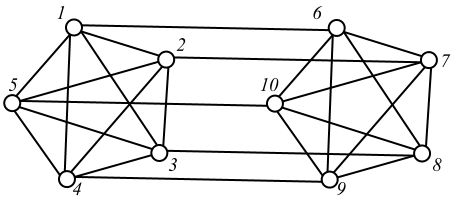
\includegraphics[scale=0.35]{imgs/k5.png}
    \captionsetup{justification=raggedright}
    \caption{Com $k=5$ temos o grafo $G$ construído pela junção dos dois grafos completos $K^1_5$ e
    $K^2_5$.~\cite{kun-et-al}}
  \end{figure}
\end{frame}

\begin{frame}
  Considere a seguinte coloração: para todo par de vértice $\{v_i,v_{i+k}\}$,
  $c(v_i)=c(v_{i+k})=i$. A coloração $c$ é \textbf{mínima} e \textbf{estável}. Então

  \begin{align*}
    &\mu_c(v)=k-1,\\
    &W(G,c)=\sum_{v\in V}\mu_c(v)=\sum_{j=1}^{|V|=2k} k-1=2k(k-1).\\
  \end{align*}

  \begin{itemize}
    \item \textbf{Estável:} Todo vértice tem $k-1$ cores diferentes em seus vizinhos.
      Cada clique $K_k$ precisa de pelo menos $k$ cores, senão não é estável.
    \item \textbf{Mínima:} Única possível aresta não apropriadamente colorida é $\{v_i,v_{i+k}\}$.
  \end{itemize}

\end{frame}

\begin{frame}
  Tome outra coloração $c'$ tal que para cada par $\{v_i,v_{i+k}\}$, $c(v_i)=i$ e $c(v_{i+k})=i+1$.
  A coloração $c'$ é \textbf{máxima}, e temos

  \begin{align*}
    &\mu_c(v)=k,\\
    &W(G,c)=\sum_{v\in V}\mu_c(v)=\sum_{j=1}^{|V|=2k} k=2k^2.\\
  \end{align*}

  \begin{itemize}
    \item \textbf{Estável:} Como é máxima, é estável.
    \item \textbf{Máxima:} Cada vértice tem $k$ vizinhos de cores diferentes e
  $\mu_c(v)=\deg(v)=k$.
  \end{itemize}
\end{frame}

\begin{frame}
  Então coloração $c$ é máxima e $c'$ mínima e estável. Portanto

  \begin{equation*}
    \PoA=\frac{\max_{c'\in C}W(G,c')}{\min_{c\in Q}W(G,c)}=\frac{2k^2}{2k(k-1)}=\frac{k}{k-1}.
  \end{equation*}

  Então $\PoA=\Theta\left(\frac{k}{k-1}\right)$.

  \hfill$\qed$
\end{frame}

\begin{frame}
  \frametitle{Colorações estritamente estáveis}
  \begin{theorem}
    Para todo $k\geq 2$, o problema de se determinar se o grafo não-direcionado $G$ tem uma
    $k$-coloração estritamente estável é NP-completo.
  \end{theorem}
\end{frame}

\begin{frame}
  \textbf{O problema está em NP\@:} dado um certificado de coloração $c$, para todo $v\in V$, verifique se
  para todo $c'(v)=i,i\in\{1,\ldots,k\}$, temos que $\mu_{c'}(v)<\mu_c(v)$.

  Vamos dividir em dois casos: $k\geq 3$ e $k=2$.

  \textbf{Reduções:}
  \begin{itemize}
    \item \textbf{Caso 1:} ($k\geq 3$) k-coloração clássica
    \item \textbf{Caso 2:} ($k=2$) 3-SAT
  \end{itemize}
\end{frame}

\begin{frame}
  \large\textbf{Caso 1:} $k\geq 3$

  \normalsize
  \begin{columns}[t]
    \begin{column}{0.9\textwidth}
      \begin{block}{Objetivo:}
        Transformar $G$ em um grafo $G'$ em que achar equilíbrio estrito equivale a achar
        $k$-coloração clássica.
      \end{block}
    \end{column}
  \end{columns}
  \vspace{0.2in}

  {\color{blue} Construção de $G'$}

  Vamos construir grafo $G'$ a partir de $G$. Copie $G$ em $G'$. Para toda aresta $e=\{u,v\}\in
  E(G')$, crie grafo $H_e$, onde $H_e$ é um grafo completo $K_{k-2}$.

  Para todo $w\in V(H_e)$, crie arestas $e_1'=\{u,w\}$ e $e_2'=\{v,w\}$ de forma a criar um clique
  $K_k$ com $H_e\cup\{u,v\}$.

  Se existe vértice isolado $v\in V(G)$ (i.e.\ $\deg(v)\leq 1$), crie uma cópia de $K_{k-1}$ e
  adicione arestas $\{v,w\}$, $w\in K_{k-1}$, em $G'$.
\end{frame}

\begin{frame}
  Vamos mostrar que uma $k$-coloração clássica em $G'$ equivale a uma $k$-coloração clássica em
  $G$, e que tal coloração equivale a um equilíbrio estrito em $G$.

  {\color{blue} Colorindo $G'$}

  Fixe uma $k$-coloração apropriada $\varphi$ de $G$. Aplique $\varphi$ em todo vértice $v\in G'$
  que veio de $G$.

  Para toda aresta $e=\{u,v\}\in E(G')$, colore $H_e$ com as $k-2$ cores diferentes de $u$ e $v$.
  Agora o clique $K_k$ de $u$ e $v$ está em equilíbrio estrito e também é uma coloração apropriada.

  Para vértices isolados, é suficiente colorir $K_{k-1}$ com as $k-1$ cores restantes diferentes da
  cor do vértice isolado.
\end{frame}

\begin{frame}
  \begin{columns}[t]
    \begin{column}{0.9\textwidth}
      \begin{block}{Objetivo:}
        Transformar $G$ em um grafo $G'$ em que \textbf{achar equilíbrio estrito equivale a achar
        $\mathbf{k}$-coloração clássica.}
      \end{block}
    \end{column}
  \end{columns}
  \vspace{0.2in}

  ($\impliedby$) Tal coloração é um equilíbrio estrito, já que para todo vértice $v\in V(G')$, $v$
  é adjacente às $k-1$ outras cores. Mudar a cor de $v$ implica em $c(v)=v(w)$, $w\in V(H_e)$, o
  que diminui $\mu_c(v)$.

  (\;$\Longrightarrow$\;) Suponha que existe equilíbrio estrito $c$ com $k$ cores em $G'$. Então
  nenhuma aresta $e=\{u,v\}$ que veio originalmente de $G$ pode ser monocromática ($c(u)=c(v)$).
  Por que?
\end{frame}

\begin{frame}
  Suponha $e=\{u,v\}$ monocromática. Então $c(u)=c(v)$. Existem $k-1$ cores a serem distribuídas em
  $H_e$. Suponha que escolhemos vértices $w\in E(H_e)$ de forma a colorir $H_e$ apropriadamente.
  Sobra uma cor $j$ não usada no clique $K_k$. Mas então $u$ tem incentivo para mudar $c(u)=j$ a
  fim de aumentar $\mu_c(u)$. Portanto não é equilíbrio. Contradição.

  Portanto, como $e$ não é monocromática, então $c$ é uma $k$-coloração clássica apropriada.

  Disso temos que \textbf{equilíbrio estrito equivale a $\mathbf{k}$-coloração clássica}, e
  portanto redução acaba para $k\geq 2$.
\end{frame}

\begin{frame}
  \large\textbf{Caso 2:} $k=2$

  \normalsize
  \begin{columns}[t]
    \begin{column}{0.9\textwidth}
      \begin{block}{Objetivo:}
        Mostrar que uma $k$-coloração estritamente estável em $G$ equivale a achar uma valoração
        verdadeira de uma fórmula em 3-CNF\@.
      \end{block}
    \end{column}
  \end{columns}
  \vspace{0.2in}

  \textbf{Passos:}
  \begin{enumerate}
    \item Tomar 3-CNF $\varphi=\cls_1\wedge\cls_2\wedge \cdots\wedge\cls_k$;
    \item Criar grafos $C_i$ que representam as conjunções $\hat{C}_i$;
    \item Mostrar que $C_i$ está em equilíbrio estrito se e somente se $\hat{C}_i$ é satisfatível
      (Lema 1);
    \item Juntar todos $C_i$ em $G$ mantendo consistência entre literais;
    \item Mostrar que $G$ está em equilíbrio estrito se e somente se $\varphi$ é satisfatível.
  \end{enumerate}
\end{frame}

\begin{frame}

  {\color{blue} 1.}

  Tome $\varphi=\cls_1\wedge\cls_2\wedge\cdots\wedge\cls_k$ uma 3-CNF\@. Queremos construir o grafo
  $G$ a partir das cláusulas disjuntivas. Para isso vamos construir os ``pedaços'' $C_i$ de $G$ de
  modo que $C_i$ corresponda a $\cls_i$.
\end{frame}

\begin{frame}

  {\color{blue} 2.}

  Vamos chamar de cláusulas \textit{gadget} os ``pedaços'' $C_i$. Os vértices extremos de $C_i$
  representam os literais de $\cls_i$. Na Figura~\ref{fig:cls}, temos a cláusula $\cls=(x\vee
  y\vee\ov{z})$.
  \begin{figure}[h]
    \centering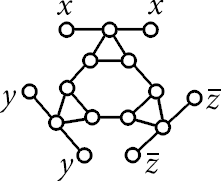
\includegraphics[scale=0.4]{imgs/clause_gadget.png}
    \captionsetup{justification=raggedright}
    \caption{\label{fig:cls} Cláusula $\cls=(x\vee y\vee\ov{z})$ representada pela cláusula
    \textit{gadget} $C$. Literais são pares de vértices e um literal ser satisfatível corresponde
    ao par ser monocromático.}
  \end{figure}
  \vspace{-0.3in}
  Vamos mostrar que se um literal é satisfatível, então o par de vértices representado em $C$ é
  monocromático. Vamos chamar este par de literal \textit{gadget}.

\end{frame}

\begin{frame}

  {\color{blue} 3.}
  \begin{lemma-cnt}
    Qualquer 2-coloração estritamente estável de uma cláusula \textit{gadget} tem um literal
    \textit{gadget} monocromático. Além disso, qualquer coloração dos literal \textit{gadgets} de
    uma cláusula \textit{gadget} que inclue um literal \textit{gadget} monocromático implica na
    cláusula \textit{gadget} estar em equilíbrio estrito.
  \end{lemma-cnt}
\end{frame}

\begin{frame}
  \frametitle{Demonstração (Lema 1)}

  Primeiro mostraremos que \textbf{toda coloração em que existe um literal \gadget{} é um
  equilíbrio estrito}. A Figura~\autoref{fig:lemma-1} enumera todas as possíveis colorações em que
  existe pelo menos um literal \gadget{} monocromático.

  \begin{figure}[h]
    \centering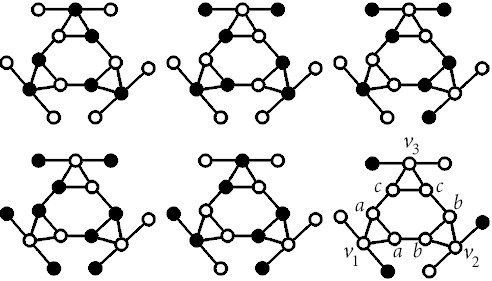
\includegraphics[scale=0.35]{imgs/lemma-1.png}
    \captionsetup{justification=raggedright}
    \caption{\label{fig:lemma-1}As cinco primeiras cláusulas \gadget{} tem algum literal \gadget{}
    monocromático. Em todos temos um equilíbrio estrito. Estas cinco cláusulas \gadget{} enumeram
    todas possíveis colorações com pelo menos um literal \gadget{} monocromático. A sexta imagem
    mostra o caso em que os literais \gadget{} não são monocromáticos.}
  \end{figure}
\end{frame}

\begin{frame}
  Agora falta mostrar que \textbf{se não existe algum literal \gadget{} monocromático na coloração,
  então ela não é estrita}.

  Suponha que exista uma coloração $c$ estritamente estável e todos literais \gadget{} são
  multicromáticos.

  {\color{gray} (desenho na lousa)}

  Chame $v_1$, $v_2$ e $v_3$ os vértices entre os literais. Chame $v_i^1,v_i^2$ os vizinhos de
  $v_i$ que não são literais. Então $c(v_i^1)=c(v_i^2)\neq c(v_i)$, senão $v_i$ não está em
  equilíbrio. Independentemente de $c(v_i)$, deve existir algum par $c(v_i^j)=c(v_p^q)$ com
  $c(v_i)=c(v_p)$. Portanto $v_i^j$ e $v_p^q$ têm incentivo para mudar, e portanto $c$ não é
  equilíbrio.

  \hfill{}$\qed$
\end{frame}

\begin{frame}
  Voltando para o Teorema 1. Mostramos passos \bcolor{1}, \bcolor{2} e \bcolor{3}. Vamos agora
  mostrar o passo \bcolor{4}:

  \normalsize
  \begin{columns}[t]
    \begin{column}{0.9\textwidth}
      \begin{block}{Passo 4:}
        Juntar todos $C_i$ em $G$ mantendo consistência entre literais.
      \end{block}
    \end{column}
  \end{columns}
  \vspace{0.2in}

  \bcolor{I.} Se uma cláusula \gadget{} $C_i$ tem o literal \gadget{} $x$ como monocromático, então
  devemos garantir que, para todo $C_j$, $i\neq j$, se o literal \gadget{} $x$ também aparecer em
  $C_j$, então ele deve ser monocromático. Da mesma forma, se $x$ não for monocromático, ele deve
  ser não monocromático em todas outras cláusulas.

  \bcolor{II.} Para $\ov{x}$, se $\ov{x}$ aparecer monocromático em uma cláusula $C_i$, então ele
  deve aparecer não monocromático em $C_j$, e vice versa.
\end{frame}

\begin{frame}
  Para \bcolor{I}, vamos construir um \textbf{literal \gadget{} de persistência}:

  \begin{figure}[h]
    \centering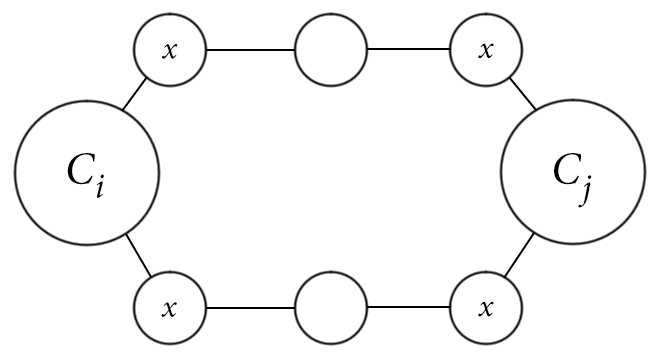
\includegraphics[scale=0.3]{imgs/persistence.png}
    \captionsetup{justification=raggedright}
    \caption{Em um literal \gadget{} de persistência, os vértices denotados por $x$ na esquerda
    fazem parte do literal \gadget{} de $C_i$, e o mesmo ocorre na direita para $C_j$. Os dois
    vértices centrais garantem que $x$ seja consistente em $C_i$ e $C_j$.}
  \end{figure}
\end{frame}

\begin{frame}
  Para \bcolor{II}, vamos construir um \textbf{literal \gadget{} de negação}:

  \begin{figure}[h]
    \centering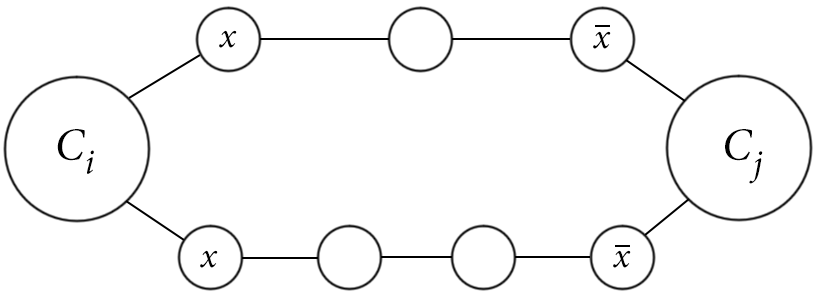
\includegraphics[scale=0.3]{imgs/negation.png}
    \captionsetup{justification=raggedright}
    \caption{Num literal \gadget{} de negação, os dois vértices inferiores garantem que as cores
    de $x$ e $\ov{x}$ sejam diferentes. Deste jeito, as duas cláusulas sempre terão colorações
    diferentes em $x$ e $\ov{x}$.}
  \end{figure}
\end{frame}

\begin{frame}

  {\color{blue}{5.}}

  Se $\varphi$ é satisfatível, então todo $\hat{C}_i$ deve ser satisfatível. Pelo Lema 1, $C_i$ é
  satisfatível se existe ao menos um literal monocromático, ou seja, tal literal é satisfatível.
  Ainda pelo Lema 1, se existe um literal monocromático, então $C_i$ está em equilíbrio estrito.

  Os literais \gadget{} de persistência e negação garantem consistência e portanto $\phi$ é
  satisfatível se e somente se é uma coloração estritamente estável.

  Como construir todos os \textit{gadgets} é polinomial, então temos uma redução polinomial de
  3-SAT\@.

  \hfill{}$\qed$
\end{frame}

%--------------------------------------------------------------------------------------------------

\section[Referências]{Referências}
\begin{frame}[t,allowframebreaks]
  \frametitle{Referências}
  \nocite{*}
  \printbibliography[]
\end{frame}

\end{document}
